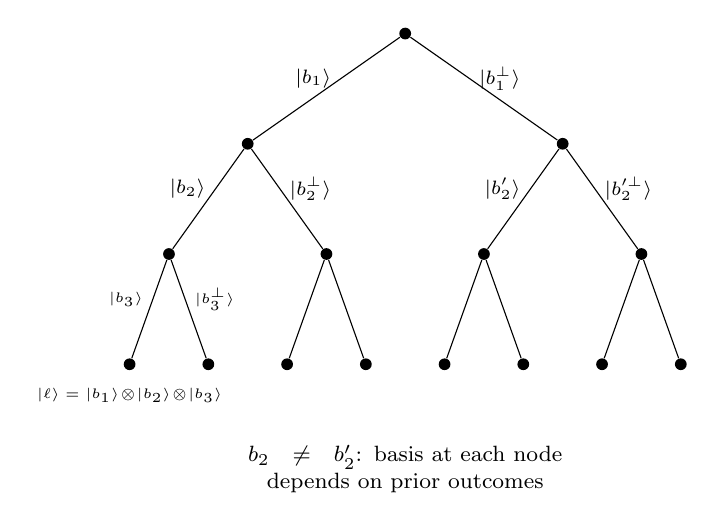
\begin{tikzpicture}[
  nd/.style={circle, fill=black, inner sep=1.5pt}]

% --- Tree nodes ---
\node[nd] (r) at (3.5, 4.2) {};
\node[nd] (a) at (1.5, 2.8) {};
\node[nd] (b) at (5.5, 2.8) {};
\node[nd] (c) at (0.5, 1.4) {};
\node[nd] (d) at (2.5, 1.4) {};
\node[nd] (e) at (4.5, 1.4) {};
\node[nd] (f) at (6.5, 1.4) {};
\foreach \i/\x in {0/0, 1/1, 2/2, 3/3, 4/4, 5/5, 6/6, 7/7} {
  \node[nd] (l\i) at (\x, 0) {};
}

% --- Root edges ---
\draw (r) -- node[left, font=\scriptsize, pos=0.4]
  {$|b_1\rangle$} (a);
\draw (r) -- node[right, font=\scriptsize, pos=0.4]
  {$|b_1^\perp\rangle$} (b);

% --- Depth 2: different bases at same level ---
\draw (a) -- node[left, font=\scriptsize, pos=0.4]
  {$|b_2\rangle$} (c);
\draw (a) -- node[right, font=\scriptsize, pos=0.4]
  {$|b_2^\perp\rangle$} (d);
\draw (b) -- node[left, font=\scriptsize, pos=0.4]
  {$|b_2'\rangle$} (e);
\draw (b) -- node[right, font=\scriptsize, pos=0.4]
  {$|b_2'^\perp\rangle$} (f);

% --- Depth 3: label leftmost pair ---
\draw (c) -- node[left, font=\tiny, pos=0.4]
  {$|b_3\rangle$} (l0);
\draw (c) -- node[right, font=\tiny, pos=0.4]
  {$|b_3^\perp\rangle$} (l1);
\draw (d) -- (l2); \draw (d) -- (l3);
\draw (e) -- (l4); \draw (e) -- (l5);
\draw (f) -- (l6); \draw (f) -- (l7);

% --- Leaf tensor product ---
\node[font=\tiny, below=5pt, anchor=north] at (l0)
  {$|\ell\rangle = |b_1\rangle
   \!\otimes\! |b_2\rangle
   \!\otimes\! |b_3\rangle$};

% --- Key property ---
\node[font=\footnotesize, anchor=north,
  text width=7cm, align=center] at (3.5, -0.9)
  {$b_2 \neq b_2'$: basis at each node
   depends on prior outcomes};

\end{tikzpicture}
